\chapter{Resultados de la Liga Endesa 2014/2015}
Este anexo consta de varias tablas con los rankings y resultados de la temporada 2014/2015 de la Liga Endesa \cite{acbresults} que hemos usado en los ejemplos del Capítulo 2.\\

\section*{Equipos participantes}

\begin{figure}[H]
	\centering
	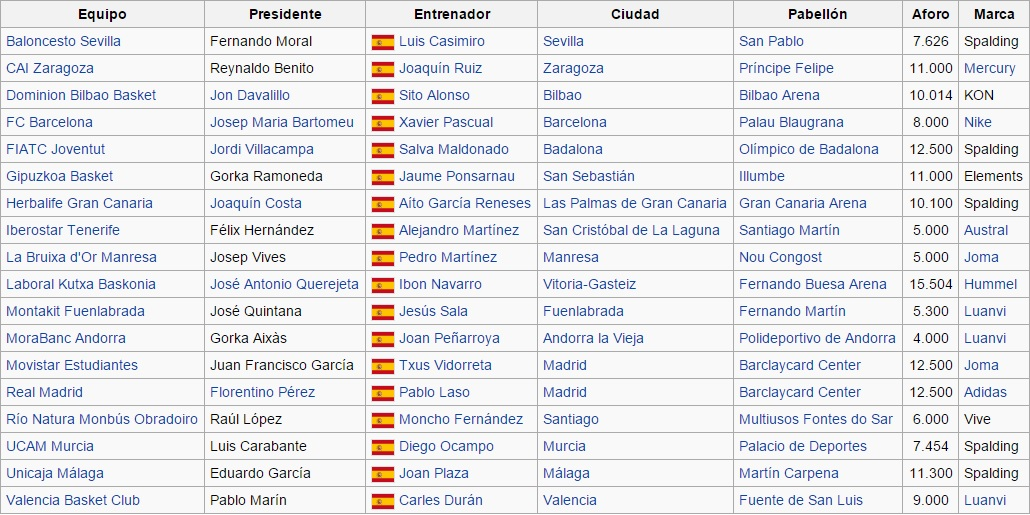
\includegraphics[scale=0.6]{images/equipos.jpg}
	\caption{Tabla de equipos.} 
\end{figure}

\section*{Ranking de la liga regular}

\begin{figure}[H]
	\centering
	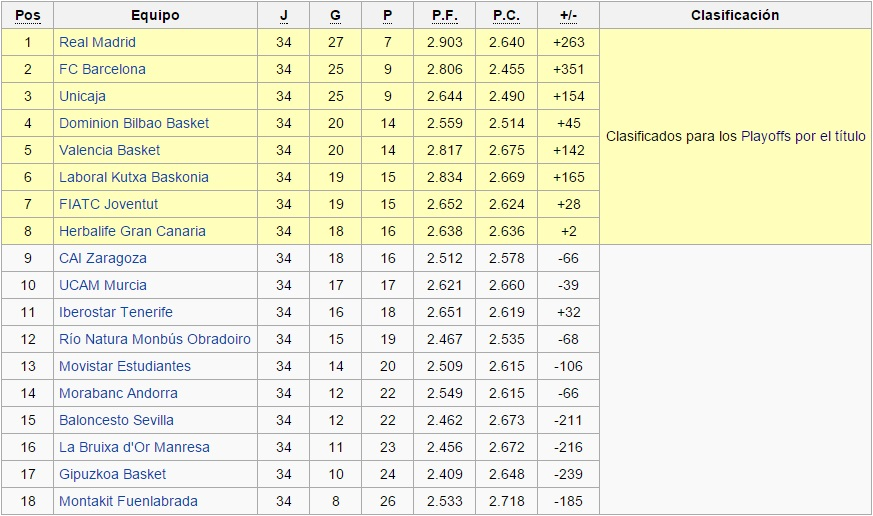
\includegraphics[scale=0.7]{images/regular.jpg}
	\caption{Ranking al finalizar la liga regular.} 
\end{figure}

\section*{Resultados de la liga regular}

\begin{figure}[H]
	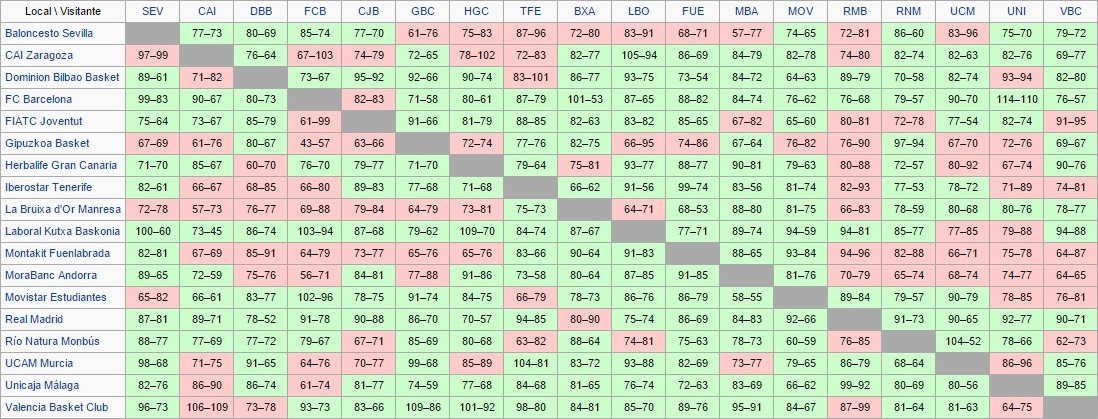
\includegraphics[scale=0.6]{images/resultados.jpg}
	\caption{Tabla de resultados de la liga regular.} 
\end{figure}

\section*{Evolución de la clasificación}

\begin{figure}[H]
	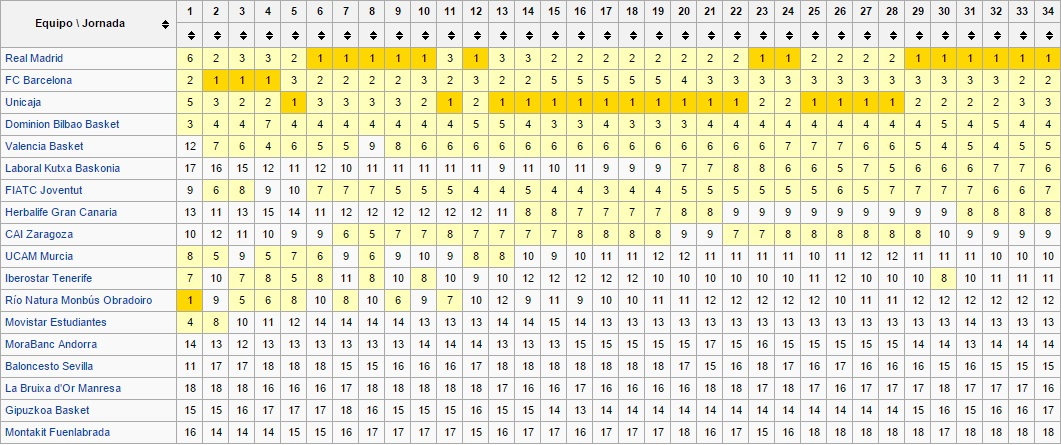
\includegraphics[scale=0.6]{images/evolucion.jpg}
	\caption{Tabla con la evolución de la clasificación.} 
\end{figure}

\section*{Playoffs}

\begin{figure}[H]
	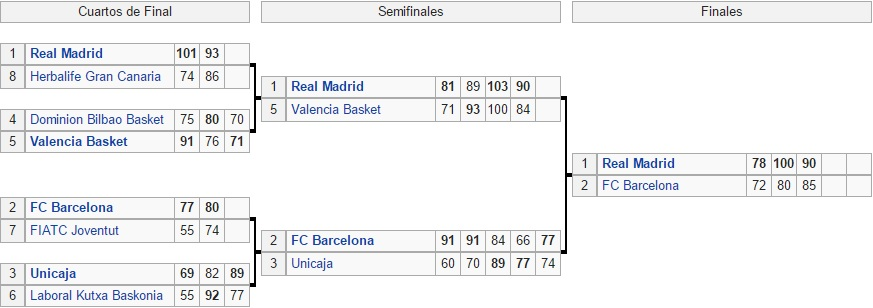
\includegraphics[scale=0.7]{images/playoffs.jpg}
	\caption{Tabla de resultados de los playoffs.} 
\end{figure}

\section*{Clasificación final}

\begin{figure}[H]
	\centering
	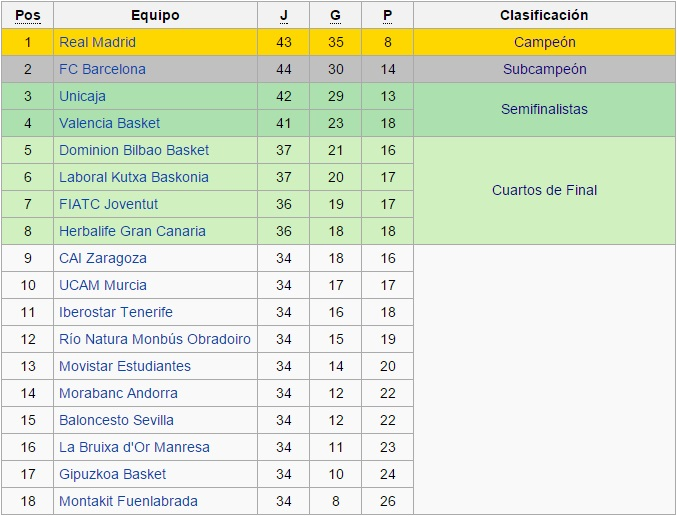
\includegraphics[scale=0.8]{images/final.jpg}
	\caption{Ranking final.} 
\end{figure}